\documentclass[lettersize,journal]{IEEEtran}
\usepackage{amsmath,amsfonts,amssymb}
\usepackage{array}
\usepackage{booktabs}
\usepackage[caption=false,font=normalsize,labelfont=sf,textfont=sf]{subfig}
\usepackage{graphicx}
\usepackage{stfloats}
\usepackage{textcomp}
\usepackage{url}
\usepackage{cite}
\hyphenation{op-tical net-works semi-conduc-tor}

\graphicspath{{journal_assets/figures/}}

\begin{document}

\title{Split-Stem Active Depth Sensing for Slit Navigation}
\author{Anonymous Manuscript}
\maketitle

\begin{abstract}
Depth images are often treated as passive geometric measurements in visual
navigation. Active stereo depth cameras violate this assumption: projector
power, exposure, and gain change the observation that a controller will receive
on the next step. This coupling is especially consequential near narrow
apertures, where a small loss of depth support can remove the very geometry
needed for collision avoidance. We study this problem in a controlled
quadrotor slit-navigation benchmark with three localized sensing regimes:
back-light glare through the opening, specular side-wall material that can
produce unstable or false depth, and low-reflectance material that weakens
active return. We introduce a split-stem active-depth policy in which the
flight branch remains adaptable while the camera branch, including its visual
stem, is fixed during final flight adaptation. This design prevents flight
optimization from moving the feature basis used by the learned camera
controller. The training pipeline combines differentiable camera-teacher
relabeling, supervised camera pretraining, DAgger-style online relabeling, and
flight-only adaptation. In held-out closed-loop evaluation over 900 episodes,
the final policy achieves 0.751 success, 0.249 collision, 0.975 depth fill, and
0.550 terminal distance, improving over fixed, random-fixed,
non-differentiable learned-camera, and blind baselines. Mechanistic analyses
show that the policy preserves scene-specific near-slit camera behavior:
glare suppresses exposure and gain, while low-reflectance material raises
them. These results support the view that active depth control can improve
navigation when sensing semantics are kept stable during policy adaptation.
\end{abstract}

\begin{IEEEkeywords}
active sensing, depth camera, slit navigation, DAgger, differentiable
perception, quadrotor navigation
\end{IEEEkeywords}

\section{Introduction}
Active depth sensing is a closed-loop problem: the policy does not merely
consume depth, it chooses the camera settings that determine what depth will be
observed next. For active stereo and structured-light sensors, projector power,
exposure, and gain modify not only brightness but the validity of the geometric
cue itself. This coupling matters most near narrow apertures, where a small
loss of usable depth can erase the very boundary needed for collision
avoidance.

We study this coupling in a minimal slit-navigation benchmark. A quadrotor
must pass through a single wall opening under three localized sensing regimes
that keep the geometry fixed while perturbing the depth observation in
physically distinct ways. Glare back-lights the opening, specular side-wall
material produces false or unstable depth, and low-reflectance material
starves the sensor of return. Because the navigation geometry is shared,
differences in performance can be traced to active sensing rather than to map
complexity or long-horizon planning.

A second failure mode appears when the camera and flight controllers share a
visual stem. Final flight optimization can improve the trajectory while moving
the feature basis used by the camera head, so the semantics of the learned
camera policy drift. We avoid that failure mode by duplicating the visual stem
and freezing the camera branch during final flight adaptation, while leaving
the flight branch trainable on the learned-camera observation distribution.

Our pipeline combines differentiable camera-teacher relabeling, camera
pretraining, DAgger-style online relabeling, and split-stem flight adaptation.
In held-out evaluation, the final policy improves success and collision over
fixed, random-fixed, non-differentiable, and blind baselines, while also
producing scene-specific camera responses near the slit. The main claim is
therefore not simply that active sensing raises fill, but that active sensing
improves navigation when camera semantics are stabilized separately from flight
optimization.

\begin{figure*}[!t]
\centering
\subfloat[Task schematic]{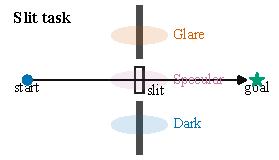
\includegraphics[width=0.31\textwidth]{panels/fig1a_task_schematic.pdf}}
\hfil
\subfloat[Active-depth loop]{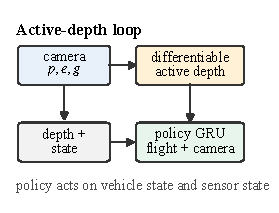
\includegraphics[width=0.31\textwidth]{panels/fig1b_active_depth_loop.pdf}}
\hfil
\subfloat[Relabel and adapt]{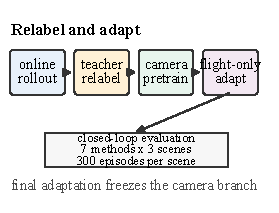
\includegraphics[width=0.31\textwidth]{panels/fig1c_relabeled_training_protocol.pdf}}
\caption{Benchmark and training protocol. The task isolates active depth
sensing in a single-wall slit-navigation environment with randomized aperture
locations and localized sensing regimes. The policy controls both flight and
camera parameters. Online states are relabeled by a differentiable camera
teacher, the camera branch is pretrained on those labels, and final flight
adaptation freezes the camera branch while updating the flight branch.}
\label{fig:system_protocol}
\end{figure*}

\section{Related Work}
Active perception frames sensing as an action rather than a passive
measurement. Early formulations argued that a robot should control its sensors
to improve the information available for subsequent decisions
\cite{bajcsy1988active,aloimonos1988active}. Later perspectives preserve the
same central idea: perception and action cannot always be optimized
independently when the action changes the measurement process
\cite{revisitingactiveperception}. Our work instantiates this principle in the
narrow but practical case of active depth sensing. The action is not only the
vehicle motion, but also the camera setting that determines the next depth
observation.

Depth-based aerial navigation commonly treats depth as a geometric input to a
controller or planner. This abstraction is reasonable when depth quality is
stable, but it hides the sensor-parameter decisions that are available on
active cameras. Automatic exposure or fixed-register operation can be adequate
in benign scenes, yet neither is explicitly optimized for the local geometric
cue that matters for a flight task. In a slit-navigation task, the relevant
quantity is not global image brightness. It is whether the aperture boundary,
adjacent wall, and through-slit return remain reliable enough for the controller
to make a collision-free decision.

The training procedure also relates to imitation learning under distribution
shift. DAgger reduces compounding error by labeling states visited by the
learner rather than only states from an initial expert distribution
\cite{ross2011dagger}. We use the same principle for the camera controller. A
differentiable camera teacher labels the states encountered by the current
learned-camera policy, and the camera head is then trained on that relabeled
online distribution. The distinctive issue in our setting is not only whether
the camera head can fit teacher labels, but whether those camera semantics
remain stable while the flight policy is later adapted.

\section{Method}
\subsection{Task Formulation}
We write scalars in italic, vectors in bold, and descriptive subscripts in
upright type. The system state at step $t$ consists of the observed depth image
$D_t^{\mathrm{obs}}$, the low-dimensional flight state $\mathbf{s}_t$, the
camera state $\mathbf{c}_t = [P_t,E_t,G_t]^\top$, and recurrent hidden state
variables. The camera channels are normalized to $[0,1]$ and correspond to
projector power $P_t$, exposure $E_t$, and gain $G_t$.

The policy is a coupled controller
\begin{equation}
    (\mathbf{u}_t, \mathbf{c}_{t+1}^{\star}, \mathbf{h}_{t+1})
    = \pi_\theta(D_t^{\mathrm{obs}}, \mathbf{s}_t, \mathbf{c}_t, \mathbf{h}_t),
\end{equation}
where $\mathbf{u}_t$ is the flight command, $\mathbf{c}_{t+1}^{\star}$ is the
target camera command, and $\mathbf{h}_t$ is the recurrent hidden state. The
applied camera state obeys a first-order update
\begin{equation}
    \mathbf{c}_{t+1} = \alpha \mathbf{c}_t + (1-\alpha)\mathbf{c}_{t+1}^{\star},
\end{equation}
with $\alpha \in (0,1)$ capturing camera latency. This matters because the
camera choice at one step changes the observation distribution available to the
next step.

The benchmark is intentionally minimal. In local scene coordinates, the vehicle
starts before a single wall and aims for a goal behind it. The slit center is
randomized laterally, and the wall is randomly rotated in the world frame so
that the policy must use local depth and state cues rather than memorize a
fixed world direction. The geometry is fixed; only the sensing regime changes.

\subsection{Differentiable Active-Depth Sensor}
The simulator first renders raw geometric depth $D_t^{\mathrm{raw}}$ from the
current pose. Raw depth depends only on scene geometry and pose, not on camera
parameters. A differentiable active-depth module then maps
$D_t^{\mathrm{raw}}$ and $\mathbf{c}_t$ to the observed depth
$D_t^{\mathrm{obs}}$, a validity mask $M_t$, and a set of quality proxies.
This separation is central: camera control cannot alter geometry, but it can
alter whether geometry is observed as usable depth.

The camera model is intentionally compact. Normalized exposure $E_t$ is mapped
to an effective integration time
\begin{equation}
    t_{\mathrm{eff}} = \mathrm{clip}(t_{\min} + t_{\mathrm{span}} E_t,\,
    t_{\mathrm{eff,min}}, t_{\mathrm{eff,max}}),
\end{equation}
and gain $G_t$ is mapped to a smooth amplification scale
\begin{equation}
    G_{\mathrm{iso}} = G_{\mathrm{base}} + G_{\mathrm{scale}}
    \frac{(G_t+\epsilon)^\gamma-\epsilon^\gamma}{(1+\epsilon)^\gamma-\epsilon^\gamma}.
\end{equation}
The constants above define the admissible operating range. Projector power and
integration time increase the active return,
\begin{equation}
    S_{\mathrm{act}} = \frac{k_a P_t t_{\mathrm{eff}}}{(D_t^{\mathrm{raw}})^2 + c_d},
\end{equation}
while exposure and gain increase the passive amplification term,
\begin{equation}
    S_{\mathrm{pass}} = k_p t_{\mathrm{eff}}\sqrt{G_{\mathrm{iso}}}.
\end{equation}
The model then combines motion blur, gain-dependent noise, range attenuation,
local depth edges, and scene masks into a continuous quality proxy, and uses a
sigmoid validity map to produce differentiable valid-depth support. The exact
physical constants are not meant to reproduce a specific camera firmware; they
are chosen to preserve the causal relation between camera parameters and depth
reliability.

\subsection{Scene-Dependent Degradation Regimes}
The three sensing regimes are localized around the slit so that geometry is
shared while sensing difficulty changes. This isolates the effect of camera
control from the effect of path geometry.
\begin{itemize}
    \item \textbf{Glare} models opening-centered back-light or infrared
    contamination. This is a saturation problem near the aperture boundary:
    excessive exposure or gain washes out the contrast that identifies the
    slit, even when projector power remains high.
    \item \textbf{Specular} models reflective side-wall material adjacent to
    the slit. This is a local reflection problem: high active power or
    unfavorable settings can produce holes, unstable edges, or false near depth
    around the reflective patches.
    \item \textbf{Dark} models low-reflectance or infrared-absorbing side-wall
    material. This is a return-starvation problem: higher exposure and gain can
    recover weak return, but they also increase blur and noise costs.
\end{itemize}
The regimes therefore require different camera behavior. A single nominal
camera setting is not expected to be uniformly optimal.

\subsection{Depth Encoding and Split-Stem Policy}
The policy consumes a two-channel depth encoding rather than raw metric depth
alone. Let $\tilde D_t$ denote the observed depth after invalid pixels are set
to zero and valid pixels are clamped to the sensor range. The encoding is
designed to preserve both near-field collision cues and through-slit
background cues:
\begin{align}
\phi_t^{\mathrm{near}} &=
\mathrm{Pool}_{\max}\left(
\mathcal{N}\left(\frac{1}{\tilde D_t}\right) \odot M_t
\right), \\
\phi_t^{\mathrm{far}} &=
\mathrm{Pool}_{\mathrm{avg}}\left(
\mathcal{N}(\tilde D_t) \odot M_t
\right),
\end{align}
where $M_t$ is the validity mask and $\mathcal{N}(\cdot)$ maps values into
$[0,1]$. The near channel emphasizes close obstacles and aperture boundaries,
while the far channel preserves the through-slit and back-wall cues that signal
free space. This decomposition is necessary because a single global depth
summary is insufficient near the slit: the controller must reason about both
edge proximity and aperture continuity.

The split-stem architecture then separates the representation used by flight
and camera control. The flight branch uses a trainable visual stem and a
recurrent controller to produce the acceleration command. The camera branch
uses a copied stem and camera-specific recurrent state to produce the next
camera target. During final flight adaptation, the camera branch and its copied
stem are frozen. The forward pass still uses the learned camera, but the flight
branch is the only part updated by gradient descent. This prevents the flight
optimizer from rewriting the feature basis that the camera policy depends on.

\subsection{Camera Teacher, Relabeling, and Flight Adaptation}
Direct end-to-end optimization of flight and camera variables can entangle two
distinct objectives: the camera must produce a useful observation, while the
flight controller must act on that observation. A camera setting that lowers a
training loss on one rollout may still destroy the semantics of the learned
camera policy or shift the observation distribution away from what the flight
branch expects. We therefore split the training into three stages.

First, a differentiable camera teacher generates supervision targets for the
visited states by optimizing a depth-health objective. The teacher favors high
fill, low blur, controlled noise, smooth transitions, and nominal recovery in
healthy regions. Second, the camera head is pretrained on rollout data.
Third, the current learned-camera policy is rolled out in closed loop, those
online states are relabeled again by the teacher, and the camera head is
updated on the relabeled distribution. This DAgger-style step is essential
because the camera semantics learned from fixed-camera rollouts are not always
stable when the observation distribution shifts.

Formally, let $\bar{\mathbf{c}}_{t+1}$ denote the teacher label for the next
camera command at step $t$. Camera pretraining and relabeling minimize a
supervised regression loss of the form
\begin{equation}
    \mathcal{L}_{\mathrm{sup}} =
    \bigl\|\mathbf{c}_{t+1}^{\star} - \bar{\mathbf{c}}_{t+1}\bigr\|_2^2,
\end{equation}
while the final flight-only stage minimizes $\mathcal{L}_{\mathrm{flight}}$
with the camera branch frozen. This is not a cosmetic choice. It explicitly
separates semantic learning of the camera from policy adaptation of the flight
controller. Without this separation, the flight optimizer can improve
short-horizon navigation while silently changing the meaning of the learned
camera outputs.

\subsection{Optimization Objectives}
The flight objective combines velocity tracking, smoothness, and collision
avoidance terms. Let $\mathcal{L}_v$ denote the velocity-tracking loss,
$\mathcal{L}_{\mathrm{acc}}$ the acceleration penalty,
$\mathcal{L}_{\mathrm{jerk}}$ the jerk penalty, and
$\mathcal{L}_{\mathrm{collide}}$ the collision-avoidance loss. With
non-negative weights $\lambda_v$, $\lambda_a$, $\lambda_j$, and $\lambda_c$,
\begin{equation}
    \mathcal{L}_{\mathrm{flight}} =
    \lambda_v \mathcal{L}_v
    + \lambda_a \mathcal{L}_{\mathrm{acc}}
    + \lambda_j \mathcal{L}_{\mathrm{jerk}}
    + \lambda_c \mathcal{L}_{\mathrm{collide}} .
\end{equation}
The camera-teacher objective balances depth health and camera operating costs.
With non-negative weights $\lambda_f$, $\lambda_b$, $\lambda_n$, $\lambda_s$,
and $\lambda_m$,
\begin{equation}
    \mathcal{L}_{\mathrm{cam}} =
    \lambda_f \mathcal{L}_{\mathrm{fill}}
    + \lambda_b \mathcal{L}_{\mathrm{blur}}
    + \lambda_n \mathcal{L}_{\mathrm{noise}}
    + \lambda_s \mathcal{L}_{\mathrm{smooth}}
    + \lambda_m \mathcal{L}_{\mathrm{nominal}} .
\end{equation}
The fill term penalizes insufficient valid depth support, blur scales with
vehicle speed and exposure time, noise scales with gain, and the nominal term
encourages recovery toward ordinary camera settings when the depth image is
already healthy. These terms are not intended to reproduce a particular camera
firmware. They provide a task-level differentiable approximation of the
tradeoffs that make active depth sensing useful for navigation.

\section{Experimental Setup}
\subsection{Evaluation Rationale}
The experiments are designed to test three linked claims. First, active camera
control should improve closed-loop navigation compared with fixed or
task-agnostic camera settings. Second, any improvement should be accompanied by
healthier depth observations, because the proposed mechanism is sensing rather
than arbitrary flight regularization. Third, the learned camera response should
be scene-specific near the slit: glare should suppress exposure and gain,
whereas low-reflectance material should increase them.

This rationale determines the organization of the evaluation. Overall success
and collision quantify the navigation outcome. Depth fill measures whether the
observation stream remains usable. Phase-wise camera statistics and
matched-pose depth sequences test whether the learned behavior is consistent
with the intended active-sensing mechanism.

\subsection{Benchmark Configuration}
Each episode lasts 60 control steps at 15 Hz, so the closed-loop horizon spans
four seconds. The raw depth renderer produces a $96 \times 72$ image, and the
policy receives a $48 \times 36$ encoded depth input. The task uses the same
wall, slit, start, and goal geometry across all sensing regimes. The slit
center is sampled laterally, and the entire scene can be randomly rotated in
yaw. This rotation means that success requires using the local depth and state
cues rather than a fixed world-frame direction.

The camera action is three-dimensional and normalized to $[0,1]^3$. The fixed
baseline uses the nominal setting. The random-fixed baseline samples a static
camera setting for each episode and keeps it fixed. Learned-camera methods
update the camera state through the smoothed camera command described above.

\begin{table}[t]
\centering
\small
\begin{tabular}{ll}
\toprule
Setting & Value \\
\midrule
Control frequency & 15 Hz \\
Episode horizon & 60 steps \\
Rendered depth resolution & $96 \times 72$ \\
Policy depth resolution & $48 \times 36$ \\
Camera action & power / exposure / gain in $[0,1]^3$ \\
Scenes & glare, dark, specular \\
Slit center & randomized laterally \\
Scene yaw & randomized \\
Teacher rollouts per scene & 4 \\
Teacher batch size & 12 \\
Teacher optimization steps & 120 \\
Camera pretraining epochs & 180, then 120 after relabeling \\
Evaluation episodes & 900 per primary method \\
\bottomrule
\end{tabular}
\caption{Core simulation, training, and evaluation settings. Evaluation uses
300 episodes per scene for each primary method.}
\label{tab:setup}
\end{table}

\subsection{Compared Policies}
The primary comparison isolates different ways of handling camera parameters.
The proposed method uses the full pipeline: differentiable camera relabeling,
DAgger-style online relabeling, split-stem camera freezing, and flight-only
adaptation. Fixed camera tests whether a single nominal setting is sufficient.
Random fixed camera tests whether merely exposing the flight policy to diverse
static camera settings explains the result. The non-differentiable learned
camera baseline tests whether a learned camera controller without the
differentiable active-sensing training signal develops the same scene-specific
behavior. The blind baseline removes depth information and provides a lower
bound on geometry-free flight.

\begin{table}[t]
\centering
\small
\begin{tabular}{lll}
\toprule
Method & Role & Description \\
\midrule
Ours & main model & split-stem learned camera with flight-only adaptation \\
Fixed & baseline & nominal constant camera setting \\
Random fixed & baseline & episode-constant random camera setting \\
Non-diff. & baseline & learned camera without differentiable sensor training \\
Blind & baseline & zero-depth controller \\
Pretrain & diagnostic & camera-pretrained policy before flight adaptation \\
DAgger & diagnostic & relabeled camera policy before flight adaptation \\
\bottomrule
\end{tabular}
\caption{Policies used in the quantitative comparison and diagnostic analysis.
Only the first five methods are primary navigation baselines; pretrain and
DAgger are included to separate camera semantics from flight adaptation.}
\label{tab:methods}
\end{table}

\subsection{Metrics and Statistical Reporting}
An episode is successful when the vehicle reaches the goal region without
collision. Collision is recorded if the trajectory intersects the wall or
violates the clearance proxy. We also report terminal distance to the goal and
the mean valid-depth fill rate. Let $\mathbf{x}_t$ denote the drone position,
$F_t$ the fraction of valid depth pixels at time $t$, and $\rho_t$ the minimum
clearance to any obstacle. We summarize
\begin{align}
\mathrm{success} &= \mathbb{1}[\|\mathbf{x}_T-\mathbf{x}_{\mathrm{goal}}\|_2 \le \delta
\ \wedge\ \neg \mathrm{collision}], \\
\mathrm{collision} &= \mathbb{1}[\exists t:\ \rho_t \le \epsilon], \\
\mathrm{fill} &= \frac{1}{T}\sum_{t=1}^{T} F_t, \\
d_{\mathrm{final}} &= \|\mathbf{x}_T-\mathbf{x}_{\mathrm{goal}}\|_2 .
\end{align}
Binary outcomes are reported with Wilson 95\% confidence intervals. Continuous
episode metrics, including fill and terminal distance, are reported with
bootstrap 95\% confidence intervals.

Camera behavior is summarized within three local phases relative to the wall,
where $x_t$ denotes the scalar local-forward component of $\mathbf{x}_t$ after
transforming the position into the wall frame:
\begin{equation}
x_t \in
\begin{cases}
\text{before}, & x_t < -0.25~\mathrm{m},\\
\text{near}, & |x_t| \le 0.25~\mathrm{m},\\
\text{after}, & x_t > 0.25~\mathrm{m}.
\end{cases}
\end{equation}
The near phase is the most important because the depth image then determines
whether the vehicle can align with the slit and avoid the wall. We report
episode-aggregated near-slit power, exposure, and gain, as well as the
glare-dark camera separation measured by the mean absolute parameter
difference. These phase-wise statistics are diagnostic rather than training
targets.

\section{Results}
\subsection{Training Curves Are a Convergence Check, Not the Main Evidence}
Figure~\ref{fig:train_curve} reports training loss, success, and collision
curves for the comparison methods. Their role is diagnostic rather than
decisive: they show that the policies reached stable regimes and that the final
flight-only run is not an incomplete optimization artifact. Final claims use
held-out closed-loop evaluation with the same episode budget and scene
distribution for every method.

For the final split-stem run, the training summary and held-out evaluation are
consistent. The training summary reports approximately 0.750 success and 0.250
collision, while held-out evaluation gives 0.751 success and 0.249 collision.
This agreement is notable because an earlier shared-stem variant produced a
larger mismatch: the camera branch appeared useful during training, but its
semantics were not stable under evaluation. The split-stem layout removes that
failure mode by fixing the camera features during flight-only adaptation. The
training curve therefore acts as a consistency check for the final system,
not as a substitute for held-out evaluation.

\begin{figure*}[!t]
\centering
\subfloat[Training loss]{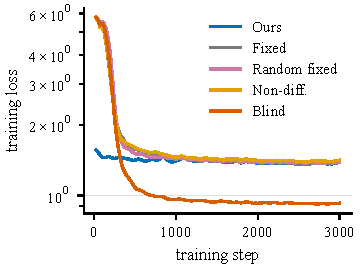
\includegraphics[width=0.32\textwidth]{panels/fig2a_training_loss.pdf}}
\hfil
\subfloat[Training success]{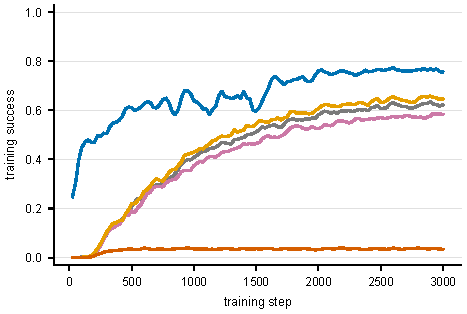
\includegraphics[width=0.32\textwidth]{panels/fig2b_training_success.pdf}}
\hfil
\subfloat[Training collision]{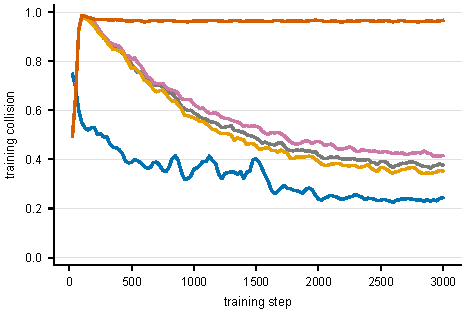
\includegraphics[width=0.32\textwidth]{panels/fig2c_training_collision.pdf}}
\caption{Training diagnostics for the comparison policies. The curves document
optimization behavior and convergence, whereas final claims use the held-out
closed-loop evaluation in Table~\ref{tab:journal_main_navigation} and
Figure~\ref{fig:navigation}.}
\label{fig:train_curve}
\end{figure*}

\subsection{Active Camera Control Improves Closed-Loop Navigation}
The primary evaluation is summarized in Table~\ref{tab:journal_main_navigation}
and Figure~\ref{fig:navigation}. The proposed policy succeeds in 0.751 of
episodes, compared with 0.667 for fixed camera, 0.627 for random fixed camera,
0.580 for the non-differentiable learned-camera baseline, and 0.032 for the
blind controller. The collision rate falls from 0.333 for fixed camera to 0.249
for the proposed policy. The improvement is not only a geometric-control
effect: depth fill rises from 0.721 under fixed camera to 0.975 under the
active policy.

\begin{table}[t]
\centering
\small
\begin{tabular}{lccccc}
\toprule
Method & Success & $\Delta$Success & Collision & Fill & $\Delta$Fill \\
\midrule
\textbf{Ours} & \textbf{0.751 [0.722,0.778]} & \textbf{+0.084} & 0.249 [0.222,0.278] & \textbf{0.975 [0.974,0.977]} & \textbf{+0.255} \\
Fixed & 0.667 [0.635,0.697] & +0.000 & 0.333 [0.303,0.365] & 0.721 [0.712,0.728] & +0.000 \\
Random fixed & 0.627 [0.595,0.658] & -0.040 & 0.373 [0.342,0.405] & 0.743 [0.733,0.752] & +0.022 \\
Non-diff. & 0.580 [0.547,0.612] & -0.087 & 0.420 [0.388,0.453] & 0.757 [0.746,0.767] & +0.036 \\
Blind & 0.032 [0.023,0.046] & -0.634 & 0.968 [0.954,0.977] & 0.622 [0.616,0.627] & -0.099 \\
\bottomrule
\end{tabular}
\caption{Primary closed-loop navigation results over 900 episodes per method. Brackets denote 95\% confidence intervals: Wilson intervals for binary outcomes and bootstrap intervals over episodes for fill. Deltas are relative to the fixed-camera baseline.}
\label{tab:journal_main_navigation}
\end{table}


\begin{figure*}[!t]
\centering
\subfloat[Success rate]{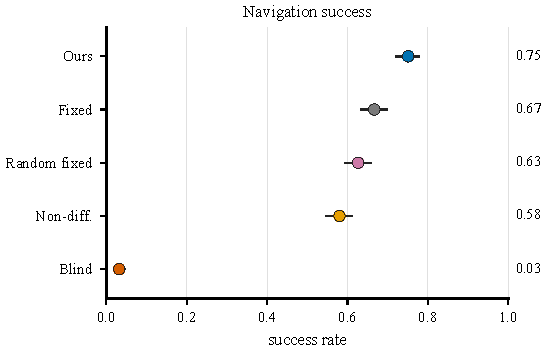
\includegraphics[width=0.48\textwidth]{panels/fig3a_navigation_success.pdf}}
\hfil
\subfloat[Depth fill]{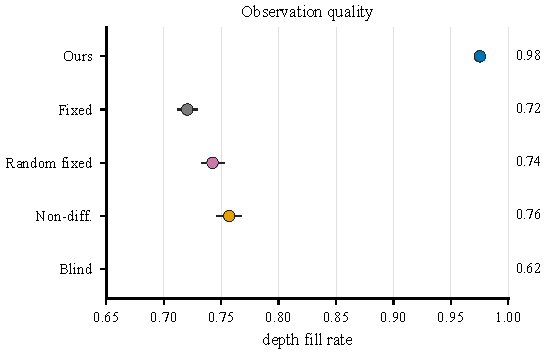
\includegraphics[width=0.48\textwidth]{panels/fig3b_depth_fill.pdf}}
\par\medskip
\subfloat[Scene-wise success gain]{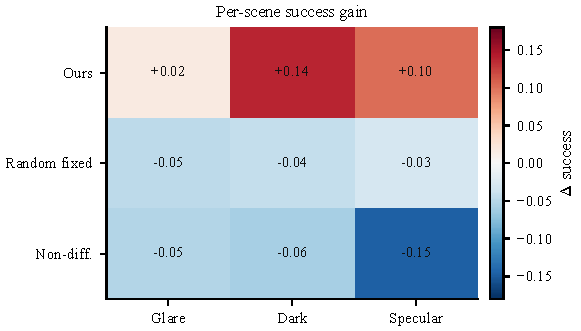
\includegraphics[width=0.48\textwidth]{panels/fig3c_scene_success_gain.pdf}}
\hfil
\subfloat[Terminal distance]{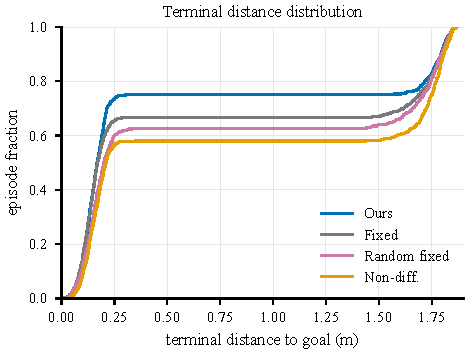
\includegraphics[width=0.48\textwidth]{panels/fig3d_terminal_distance_ecdf.pdf}}
\caption{Closed-loop navigation performance. The proposed split-stem active
camera policy improves success while maintaining substantially higher valid
depth fill than fixed, random-fixed, non-differentiable learned-camera, and
blind baselines.}
\label{fig:navigation}
\end{figure*}

The joint improvement in success and fill is the key point. A gain in success
without a gain in fill could be explained by a more conservative policy or a
different trajectory distribution. A gain in fill without a gain in success
would mean that the camera learned to recover pixels that the controller cannot
use. The proposed method is the only learned-camera variant that improves both
metrics over the fixed baseline. Random-fixed and non-differentiable baselines
do increase fill, but they do not improve success. That separation matters:
the recovered pixels must be scene-conditioned and must appear at the right
part of the aperture to affect collision avoidance. The final policy therefore
improves the sensing stream and then converts that improved observation into
higher success.

\subsection{Scene-Level Results Show Where the Gain Occurs}
The scene breakdown in Table~\ref{tab:journal_scene_breakdown} reveals that the
benefit is not uniform across regimes. Dark material benefits the most because
it is fundamentally a return-starvation problem: additional exposure and gain
can recover weak returns without erasing the slit boundary, so the extra fill
translates cleanly into more successful traversals. Specular scenes are
intermediate because the dominant failure mode is local reflection and edge
instability around the side-wall patches; the learned camera can damp that
instability, but it cannot eliminate it. Glare is the hardest regime because it
is a saturation problem near the aperture boundary. The camera can suppress
overexposure and recover a large amount of valid depth, yet the remaining error
is concentrated exactly where the controller needs clean contrast, so the gain
in success is smaller than the gain in fill.

\begin{table}[t]
\centering
\footnotesize
\renewcommand{\arraystretch}{1.12}
\setlength{\tabcolsep}{9pt}
\begin{tabular}{@{}lccc@{}}
\toprule
Method & \shortstack{Glare\\Succ./Fill} & \shortstack{Dark\\Succ./Fill} & \shortstack{Specular\\Succ./Fill} \\
\midrule
\textbf{Ours} & \textbf{0.67/0.96} & \textbf{0.82/0.98} & \textbf{0.76/0.99} \\
Fixed & 0.65/0.69 & 0.68/0.70 & 0.66/0.77 \\
Random fixed & 0.61/0.69 & 0.64/0.73 & 0.63/0.80 \\
Non-diff. & 0.60/0.67 & 0.62/0.67 & 0.52/0.93 \\
Blind & 0.03/0.60 & 0.03/0.59 & 0.03/0.68 \\
\bottomrule
\end{tabular}
\caption{Scene-wise success and depth-fill rates.}
\label{tab:journal_scene_breakdown}
\end{table}


This asymmetry is the mechanism-level result. Dark and glare both gain fill,
but only dark converts most of that gain into success. The difference is
physical rather than statistical: dark suppresses return that can be recovered
by integration and gain, whereas glare corrupts the contrast at the aperture
itself. Fill is therefore necessary but not sufficient; the controller also
needs the recovered pixels to preserve the slit boundary.

\subsection{The Learned Camera Implements Scene-Specific Near-Slit Behavior}
Table~\ref{tab:journal_camera_response} and Figure~\ref{fig:camera_mechanism}
test whether the learned camera has interpretable active-sensing semantics. In
the near-slit phase, the proposed policy uses high power but low exposure and
gain in glare, high exposure and gain in dark material, and a lower-power
intermediate setting in specular scenes. The direction of change is physically
coherent. In glare, suppressing exposure and gain protects the aperture
boundary from saturation. In dark material, increasing exposure and gain
compensates for weak return. Specular scenes sit between those extremes, with
lower power to avoid reflective hotspots and moderate exposure and gain to
stabilize the adjacent patches. The glare-dark separation reaches 0.412 with a
narrow confidence interval, whereas fixed camera, non-differentiable learned
camera, and blind control remain at or near zero. Random fixed camera has small
separation because its sampled settings differ between episodes, but that
separation is not scene-conditional and remains far below the proposed policy.

\begin{table*}[t]
\centering
\footnotesize
\renewcommand{\arraystretch}{1.12}
\begin{tabular*}{\textwidth}{@{\extracolsep{\fill}}lcccc@{}}
\toprule
Method & \shortstack{Glare\\$P/E/G$} & \shortstack{Dark\\$P/E/G$} & \shortstack{Specular\\$P/E/G$} & \shortstack{Glare--dark L1\\(95\% CI)} \\
\midrule
\textbf{Ours} & \textbf{0.731/0.088/0.120} & \textbf{0.665/0.694/0.683} & \textbf{0.408/0.366/0.381} & \textbf{0.412 [0.406,0.417]} \\
Fixed & 0.500/0.500/0.500 & 0.500/0.500/0.500 & 0.500/0.500/0.500 & 0.000 [0.000,0.000] \\
Random fixed & 0.523/0.522/0.467 & 0.541/0.521/0.453 & 0.526/0.504/0.455 & 0.011 [0.006,0.039] \\
Non-diff. & 0.413/0.373/0.508 & 0.413/0.373/0.507 & 0.408/0.365/0.510 & 0.000 [0.000,0.002] \\
Pretrain & 0.714/0.061/0.103 & 0.682/0.724/0.709 & 0.392/0.352/0.365 & 0.433 [0.427,0.439] \\
DAgger & 0.728/0.069/0.109 & 0.676/0.727/0.708 & 0.392/0.360/0.368 & 0.436 [0.426,0.445] \\
Blind & 0.500/0.500/0.500 & 0.500/0.500/0.500 & 0.500/0.500/0.500 & 0.000 [0.000,0.000] \\
\bottomrule
\end{tabular*}
\caption{Near-slit camera commands and glare--dark separation.}
\label{tab:journal_camera_response}
\end{table*}


\begin{figure*}[!t]
\centering
\subfloat[Near-slit camera fingerprint]{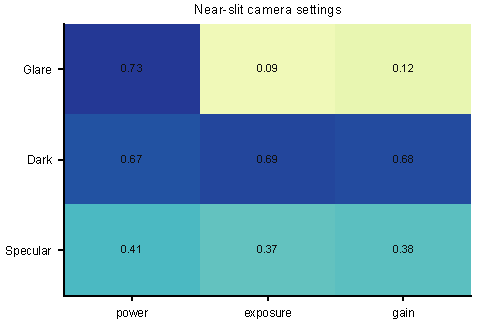
\includegraphics[width=0.31\textwidth]{panels/fig4a_camera_fingerprint.pdf}}
\hfil
\subfloat[Exposure--gain response]{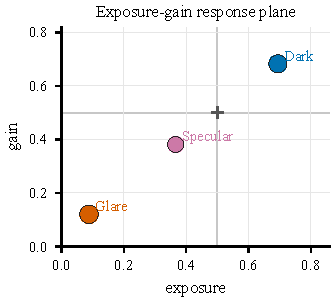
\includegraphics[width=0.31\textwidth]{panels/fig4b_exposure_gain_plane.pdf}}
\hfil
\subfloat[Local degradation]{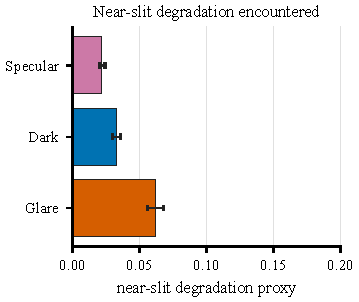
\includegraphics[width=0.31\textwidth]{panels/fig4c_near_slit_degradation.pdf}}
\par\medskip
\subfloat[Profiles across the wall frame]{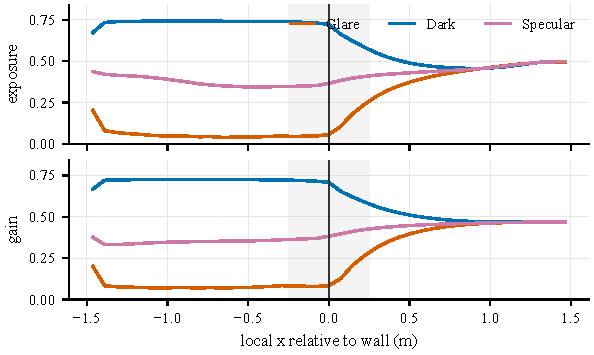
\includegraphics[width=0.62\textwidth]{panels/fig4d_exposure_gain_profiles.pdf}}
\hfil
\subfloat[Successful trajectory envelopes]{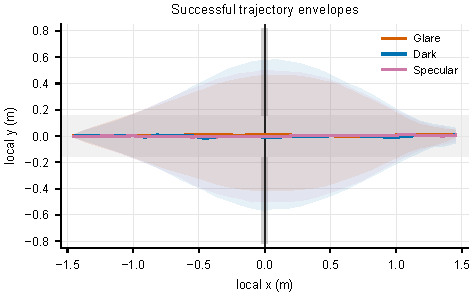
\includegraphics[width=0.34\textwidth]{panels/fig4e_trajectory_envelopes.pdf}}
\caption{Near-slit active-camera mechanism. The final policy produces
scene-specific camera settings near the wall: glare suppresses exposure and
gain, dark material increases them, and specular material uses a distinct
lower-power regime. The same figure relates these camera settings to local
degradation strength and successful trajectory envelopes.}
\label{fig:camera_mechanism}
\end{figure*}

This analysis is important because a higher fill rate alone would not be
enough to claim active sensing. A controller could push all parameters toward
one extreme and improve fill in some cases without learning the regime
structure. The near-slit fingerprints show the opposite: the policy changes its
settings in a scene-conditional way, and the directions match the sensor
model. The non-differentiable baseline is revealing because it can raise fill
without reproducing the same scene-conditional motion, which explains why its
navigation performance remains weaker.

\subsection{Matched-Pose Depth Sequences Isolate the Camera Effect}
The qualitative depth sequences in Figure~\ref{fig:depth_seq} provide a visual
counterpart to the scalar metrics. Each panel re-renders observed depth at
matched poses, using the same raw geometric depth but different camera settings.
This matched-pose construction matters because it separates camera effects from
trajectory effects. If two methods see different depth images at different
poses, the difference could come from either motion or sensing. Here the pose is
held fixed, so changes in observed depth are attributable to camera parameters
under the same geometry.

\begin{figure*}[!t]
\centering
\subfloat[Glare]{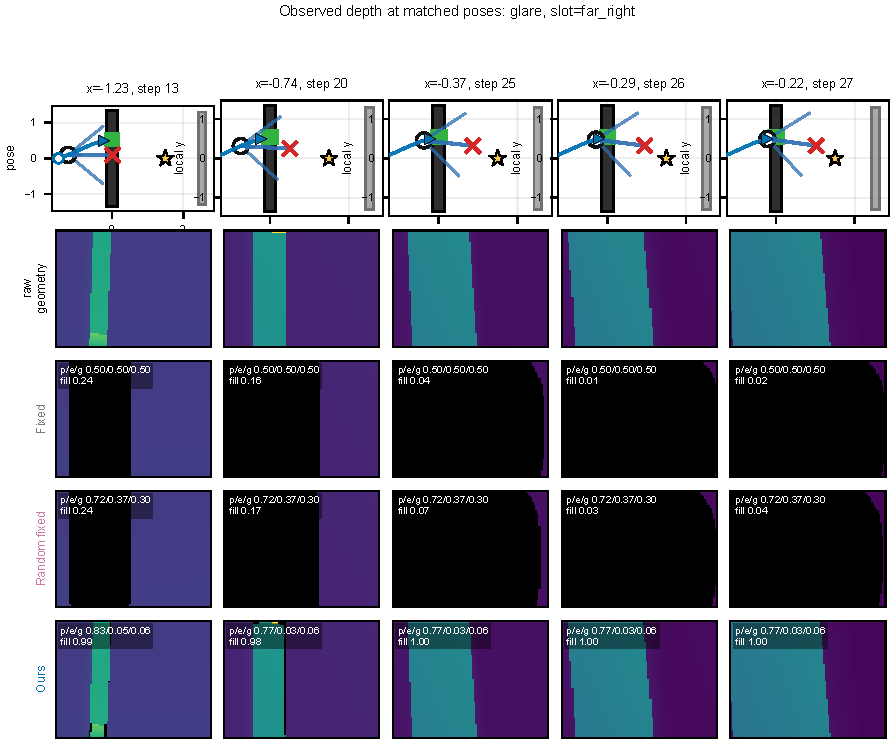
\includegraphics[width=0.32\textwidth]{fig5_depth_observation_sequence_glare.pdf}}
\hfil
\subfloat[Dark]{\includegraphics[width=0.32\textwidth]{fig5_depth_observation_sequence_dark.pdf}}
\hfil
\subfloat[Specular]{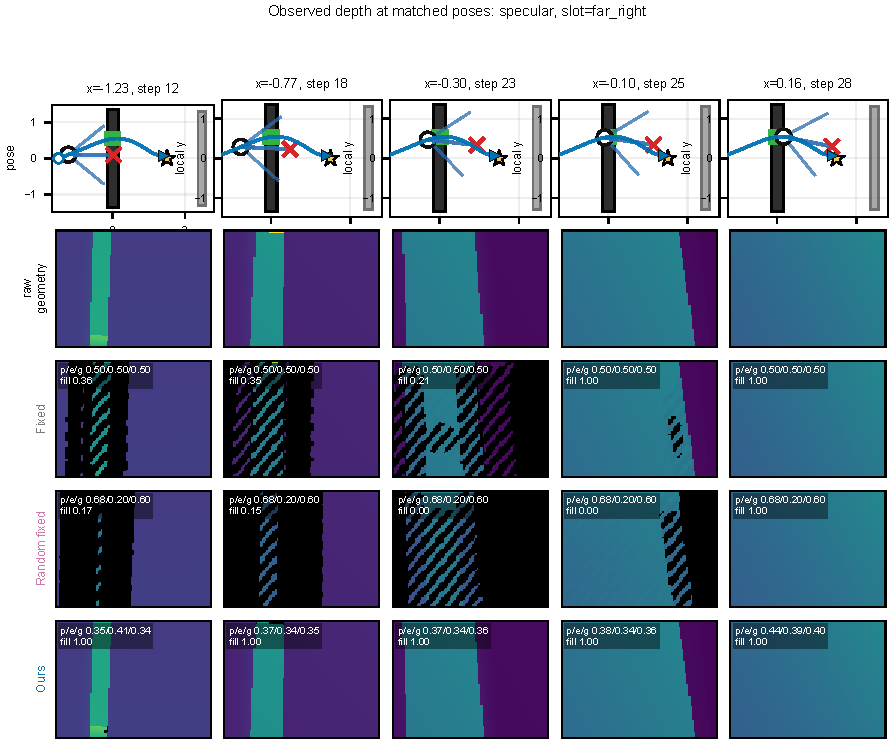
\includegraphics[width=0.32\textwidth]{fig5_depth_observation_sequence_specular.pdf}}
\caption{Matched-pose depth observation sequences rendered along the same rollout
poses. The raw geometry is fixed; only the camera parameters change the observed
depth.}
\label{fig:depth_seq}
\end{figure*}

The sequences explain why fill alone is not the whole story. In glare, nominal
camera settings leave invalid regions around the opening, whereas the learned
camera preserves usable aperture structure by suppressing exposure and gain.
In dark material, the learned camera recovers return that would otherwise be
weak under nominal settings. In specular material, the gain is more subtle
because fixed camera already preserves more geometry, but the active policy
still maintains a cleaner observation than the random-static setting. The
recovered pixels are therefore not only more numerous; they are better aligned
with the aperture and side-wall structures that determine the flight decision.

\subsection{Camera Relabeling and Flight Adaptation Are Complementary}
Figure~\ref{fig:dagger_diag} separates two questions that are easy to conflate.
The first is whether the camera branch has learned meaningful scene-dependent
semantics. The second is whether the flight branch can use the resulting
observation distribution to navigate. Camera pretraining and DAgger relabeling
answer the first question. They recover clear glare-dark camera separation in
online rollouts, with high exposure and gain in dark material and low exposure
and gain in glare. However, these camera-only policies do not answer the
second question: they produce meaningful camera semantics, but the flight
controller has not yet adapted to the resulting observation stream.

This is expected. A learned camera changes the distribution of depth images
seen by the controller. Even if the camera is semantically correct, the flight
policy still has to adapt to the new observation stream. The final flight-only
stage performs that adaptation while freezing the camera branch. The result is
that the final policy preserves the DAgger-learned camera separation while
achieving substantially higher navigation success than the camera-only
diagnostic policies. The diagnostic checkpoints are therefore useful rather
than contradictory: they show that camera semantics can be learned before they
become operationally useful for closed-loop flight.

\begin{figure*}[!t]
\centering
\subfloat[Camera-semantics recovery]{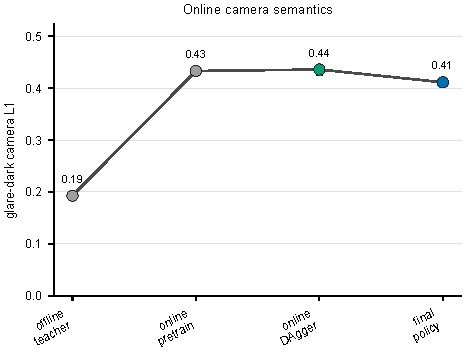
\includegraphics[width=0.32\textwidth]{panels/fig6a_camera_semantics_progress.pdf}}
\hfil
\subfloat[Dark--glare parameter changes]{\includegraphics[width=0.32\textwidth]{panels/fig6b_dark_glare_parameter_delta.pdf}}
\hfil
\subfloat[Separation versus success]{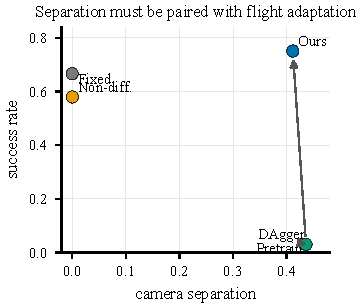
\includegraphics[width=0.32\textwidth]{panels/fig6c_separation_success.pdf}}
\caption{Camera relabeling and flight adaptation are complementary. Relabeling
restores scene-specific camera semantics, but competitive navigation requires
an additional flight-only adaptation stage under the learned-camera observation
distribution.}
\label{fig:dagger_diag}
\end{figure*}

\section{Discussion}
\subsection{What the Evidence Supports}
The experiments support a focused claim: in this controlled slit-navigation
benchmark, task-aware active depth sensing improves closed-loop flight when the
camera semantics learned from a differentiable teacher are preserved during
final policy adaptation. The evidence is not based on a single metric. Success
improves relative to the primary baselines, collision decreases, depth fill
increases substantially, near-slit camera settings separate according to scene
regime, and matched-pose renderings show that those settings change the
observed depth image under the same geometry.

The regime asymmetry is the most informative part of that result. Dark scenes
improve the most in success because they are return-starvation problems:
additional exposure and gain recover weak returns without destroying the slit
boundary. Glare improves more in fill than in success because it is a
saturation problem: the camera can recover valid pixels, but the aperture edge
is still vulnerable to contamination. Specular scenes sit between those
extremes because local reflection creates holes and edge drift that the camera
can mitigate but not completely remove. The benchmark therefore shows not just
that active sensing helps, but that it helps for physically meaningful reasons.

The split-stem design is important for this conclusion. The camera branch is
not merely another head attached to a representation that continues to move
during flight training. It has its own copied visual pathway and camera-specific
modules, and these components are frozen during flight-only adaptation. This
keeps the meaning of the camera head stable while allowing the flight branch to
adapt to the learned-camera depth stream.

\subsection{What the Evidence Does Not Claim}
The result should not be read as a claim that active camera control solves
general aerial navigation or that depth fill alone determines success. The
benchmark is intentionally narrow, and the strongest navigation gain occurs in
the dark-material regime. Glare remains difficult: the active camera improves
fill substantially, but success improves only modestly. This distinction is
important. A valid depth pixel is useful only if it preserves the task-critical
aperture cue at the right time and location. Global fill is therefore a
necessary but incomplete indicator of navigation quality. The random-fixed and
non-differentiable baselines make the same point from the negative side: they
can raise fill, but if the recovered pixels are not scene-conditioned, the
navigation policy does not improve.

Nor should the pretrain and DAgger diagnostic policies be interpreted as failed
camera controllers. Their purpose is to show that camera semantics can be
learned and preserved. Their low navigation success demonstrates a different
point: the flight controller must be adapted after the camera changes the
closed-loop observation distribution.

\subsection{Limitations and Threats to Validity}
The study is simulation-only. The sensor model is designed to preserve the
causal relationships among power, exposure, gain, motion blur, noise, and
localized depth degradation, but it is not a pixel-accurate model of any
specific commercial depth camera. Transferring the method to hardware would
require calibration of the sensor parameters, validation under real lighting
and material conditions, and safeguards for register limits and temporal camera
latency.

The evaluation also uses a single training seed. The held-out episode count is
large enough to estimate closed-loop performance for the trained checkpoints,
but it does not measure variance across independently trained policies. A
stronger future study would report multiple training seeds, additional slit
widths, and hardware-in-the-loop or real-robot trials. These extensions are
outside the scope of the present benchmark, whose purpose is to isolate the
mechanism of active depth sensing under controlled degradation.

\section{Conclusion}
We presented a split-stem active depth sensing pipeline for quadrotor
slit navigation. The method treats camera parameters as part of the closed
loop, learns camera behavior from differentiable teacher relabeling, and then
adapts the flight branch while freezing the camera branch. In held-out
evaluation, the final policy improves success and depth fill over fixed,
random-fixed, non-differentiable learned-camera, and blind baselines. The
mechanism analysis shows that this improvement is accompanied by interpretable
scene-specific camera behavior near the slit. These results indicate that
active depth control is most effective when sensing semantics and flight
adaptation are treated as coupled but separately stabilized parts of the policy.

\bibliographystyle{IEEEtran}
\bibliography{ref}

\end{document}
